\documentclass[a4paper,twoside, openright,12pt]{report}
\usepackage{psfrag,amsbsy,graphics,float}
\usepackage[pdftex]{graphicx, color}
\usepackage[latin1]{inputenc}
\usepackage{verbatim} 
% Eigene packages f�r subfigures
\usepackage{caption}
\usepackage{subcaption}
\usepackage{appendix}
\usepackage{algorithm2e}
\usepackage{url}

\usepackage{lipsum}
\usepackage[nohyperlinks]{acronym}

\usepackage{textcomp}
\usepackage{gensymb}

\usepackage{amsmath}
\DeclareMathOperator*{\argmax}{arg\,max}



%_______Kopf- und Fu�zeile_______________________________________________________
\usepackage{fancyhdr}
\pagestyle{fancy}
%um Kopf- und Fu�zeile bei chapter-Seiten zu reaktivieren
\newcommand{\helv}{%
   \fontfamily{phv}\fontseries{a}\fontsize{9}{11}\selectfont}
\fancypagestyle{plain}{	
	\fancyfoot{}% keine Fu�zeile
	\fancyhead[RE]{\helv\leftmark}% Rechts auf geraden Seiten=innen; in \leftmark stehen \chapters
	\fancyhead[LO]{\helv\rightmark}% Links auf ungeraden Seiten=au�en;in \rightmark stehen \sections
	\fancyhead[RO,LE]{\thepage}}%Rechts auf ungeraden und links auf geraden Seiten
%Kopf- und Fu�zeile f�r alle anderen Seiten
\fancyfoot{}
\fancyhead[RE]{\helv\leftmark}
\fancyhead[LO]{\helv\rightmark}%alt:\fancyhead[LO]{\itshape\rightmark}
\fancyhead[RO,LE]{\thepage}
%________________________________________________________________________________


%_Definieren der R�nder und L�ngen__________
\setlength{\textwidth}{15cm}
\setlength{\textheight}{22cm}
\setlength{\evensidemargin}{-2mm}
\setlength{\oddsidemargin}{11mm}
\setlength{\headwidth}{15cm}
\setlength{\topmargin}{10mm}
\setlength{\parindent}{0pt} % Kein Einr�cken beim Absatz!!
%___________________________________________


%_______Titelseite__________________________________________
\begin{document}
\pagestyle{empty}
\enlargethispage{4.5cm} %Damit das Titelbild weit genug unten ist!
\begin{center}
\phantom{u}
\vspace{0.5cm}
\Huge{\sc Poppy Arm Control \\ using \\ Deep Reinforcement Learning}\\
\vspace{1.5cm}

\large{REPORT for \\
PROBLEM DESCRIPTION and MODELING \\

\vspace{1.5cm}

by\\          

\vspace{0.4cm}

Mohamed Fares Abid \\						
Bo Huang \\
Maxime Kirgo \\					
R\'emi Laumont \\
Dominik Meinzer\\
Jiawen Xu \\
					
\vspace{0.5cm}

\vspace{1.5cm}
Applied Reinforcement Learning \\
Lehrstuhl f\"ur\\
DATENVERARBEITUNG\\
Technische Universit\"at M\"unchen\\
\vspace{0.3cm}
Prof. Dr.-Ing. Klaus Diepold}
\end{center}

%____________________________________________________________
\newpage

\pagestyle{fancy}

%_________Inhaltsverzeichnis__________________________
\tableofcontents 
%_____________________________________________________

%_________Einleitung__________________________________
\chapter{Introduction}
In recent years, model-free \ac{DRL} using Q-learning has accomplished impressive results in achieving superhuman capabilities in Atari 2600 games \cite{mnih2013playing, mnih2015human, mnih2016asynchronous}. Besides the game domain, many Deep Q-learning methods have been developed for control in Robotics \cite{gu2016deep, gu2016offpolicy}, where the robots learn in little time, without demonstration or human interaction, how to open a door. Q-learning \cite{watkins1992q, watkins1989learning} is a \textit{model-free} \ac{TD} method that can be used to learn an optimal policy to any given task. The method can learn in an \textit{off-policy} manner, i.e. an optimal policy is learned regardless of the current agent's behavior. The model-free property allows to learn the underlying model by sampling from the environment and the possibility to train off-policy makes the method data efficient \cite{gu2016offpolicy}. However, a basic, iterative learning approach, where a policy is learned in a tabular fashion for every state-action pair, is often impractical in real-world applications \cite{kober2012reinforcement}. Using a non-linear function approximator, like a deep \ac{NN} and feeding enough data into the network produces good feature representations which are learned directly from the data. As a consequence, deep \acp{NN} have become a popular function approximator and were successfully applied in complex situations. \\
Inspired by the aforementioned works and the will to use and learn about a very basic algorithm in \ac{DRL}, we aim to control the arm motion of Poppy, a humanoid robot, in this work using the \ac{DQN} algorithm. Applying \ac{DRL} in this project will give us necessary experience for future projects, even outside of this lecture. \\
In the following report, we will first concretize our the problem of manipulation of the Poppy robot. Second, we explain our modeling of the problem and how we can simplify the problem to make learning easier and faster.

%____________________________________________________
%_____Hauptteil______________________________________
\chapter{Problem Description}

\begin{figure}[H]
	\centering
	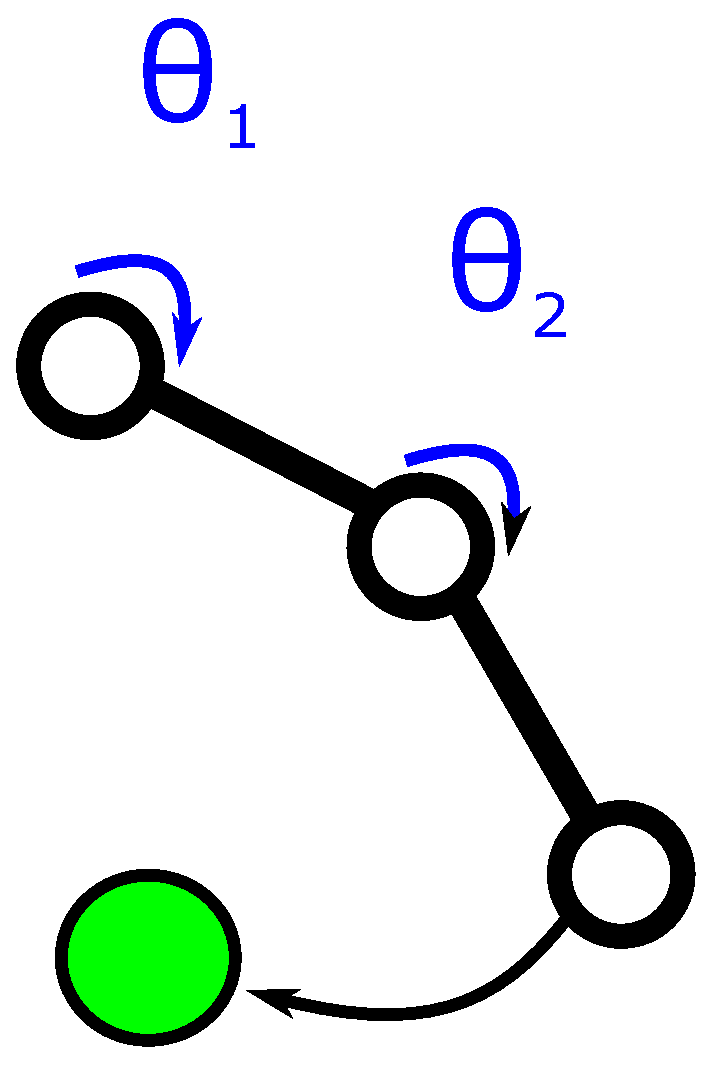
\includegraphics[width=0.2\textwidth]{reportpics/task.eps}
	\caption{Arm Control Task}
	\label{fig:task}
\end{figure}

In this work, we use a humanoid robot, called Poppy. Typical tasks for humanoid robots with many degrees of freedom is to learn motion control. In our case, we will focus on arm motion. The problem of controlling a robotic manipulator can often be solved by using \acp{IK}, but have drawbacks like singularities, joint limitations and maybe unknown kinematic parameters, such as arm lengths. However, manipulation provides us with a simple example to use the \ac{DQN} method. In theory, Q-learning allows us to learn any task based on the model-free property. In addition, using \acp{NN} allows us to learn necessary features for accomplishing the task instead of manually generating good features, which can be very useful for more difficult and complicated problems. Another advantage of the \ac{NN} is the generalization inside the action-state space, because reaching and trying all different configurations infinitely often to learn good Q-values is impossible, even in a simple manipulation example. Nevertheless, the \ac{DQN} algorithm should be able to learn a simple reaching task, i.e. how to control the arm to a given target position, while the robot will be able to cope with singularities, joint limitations and unknown arm lengths. Based on the idea of Q-learning, we can even extend the task to different scenarios, such as using both arms, drawing triangles or other shapes, depending on the time of the project. Although the problem of arm motion seams simple, we would like to emphasize that the \ac{DRL} technique, the \ac{DQN} algorithm is not, as non-linear function approximators, such as deep \ac{NN} often tend to diverge in \ac{DRL}. Achieving a smart agent in the end will be the most challenging part of the project. Mnih et al.~\cite{mnih2015human} proposed the \ac{DQN} algorithm, including the ideas of a replay memory and a target network, which will be the starting point for our algorithm. In addition, we introduce our own exploration policy, because $\epsilon$-greedy is not suitable for exploration on real hardware and will not result in a short learning time. The exploration is based on an \acp{IK} approach to guide the robot arm into the direction of the target and explore randomly around this trajectory. The details will be explained in Sec. \ref{sec:modeling}. Finally, we will have to tune many hyperparameters in order to make the robot move as we expect.

\chapter{Modeling} \label{sec:modeling}
Due to the short project time, we want to start with a very simplified version of the problem. Consequently, we focus on only arm motion of the robot. Additionally, we decrease the degrees of freedom of the Poppy arm from 4 to 2, see Fig. \ref{fig:poppy_2dof}. This means that we will restrict the control to motors \textit{l\_shoulder\_x} and \textit{l\_elbow\_y}, called in the following $\theta_1$ and $\theta_2$ respectively. Motor l\_shoulder\_y is set to $-90\degree$ and motor l\_arm\_z is hold at $0\degree$ in order to allow movements of the hand only in the x-axis (sideways) and y-axis (forward/backwards). This restriction should help us to learn a reasonable behavior of the robot arm in shorter training time. \\
The original \ac{DQN} algorithm uses images as input to the Q-Network and discrete joystick actions. In order to simplify the state space, we will not use images as input, but a description of the robot and the environment in only 6 states. Nevertheless, this description fulfills the Markovian property. These 6 states consist of the two joint angles of the robot arm $\vec{\theta} = [\theta_1, \theta_2]$, the end-effector position in the x-y plane $\vec{x}_{arm} = [x_{arm}, y_{arm}]$ and the goal position in the x-y plane $\vec{x}_{goal} = [x_{goal}, y_{goal}]$. This means that our state $s$ is:
\begin{equation}
s = [x_{arm}, y_{arm}, \theta_1, \theta_2, x_{goal}, y_{goal}]
\end{equation} 
where the arm joint angles $\theta_i$ can be measured by the internal sensors of the robot, the position of the end-effector can be computed by simple forward kinematics and the goal position is set by ourselves manually at the beginning of the project. If everything is working out as planned, we may include vision to determine the goal. The action space in our project is planned to be 4 discrete actions. The agent controls two motors and can move each motor with $\pm1\degree$. A larger action space will be considered during the experiments, but may be harder to train. The reward signal $r$ is designed as the negative distance between the end-effector position and the goal position, i.e.
\begin{equation}
r = -\left\Vert\left( \vec{x}_{arm} - \vec{x}_{goal} \right) \right\Vert^2
\end{equation}
This reward design is punishing the agent more when moving away from the target and punishing the agent less when approaching the target. Additionally, punishing the agent in every step is forcing the agent to get to the goal as fast as possible.\\

\begin{figure}
	\centering
	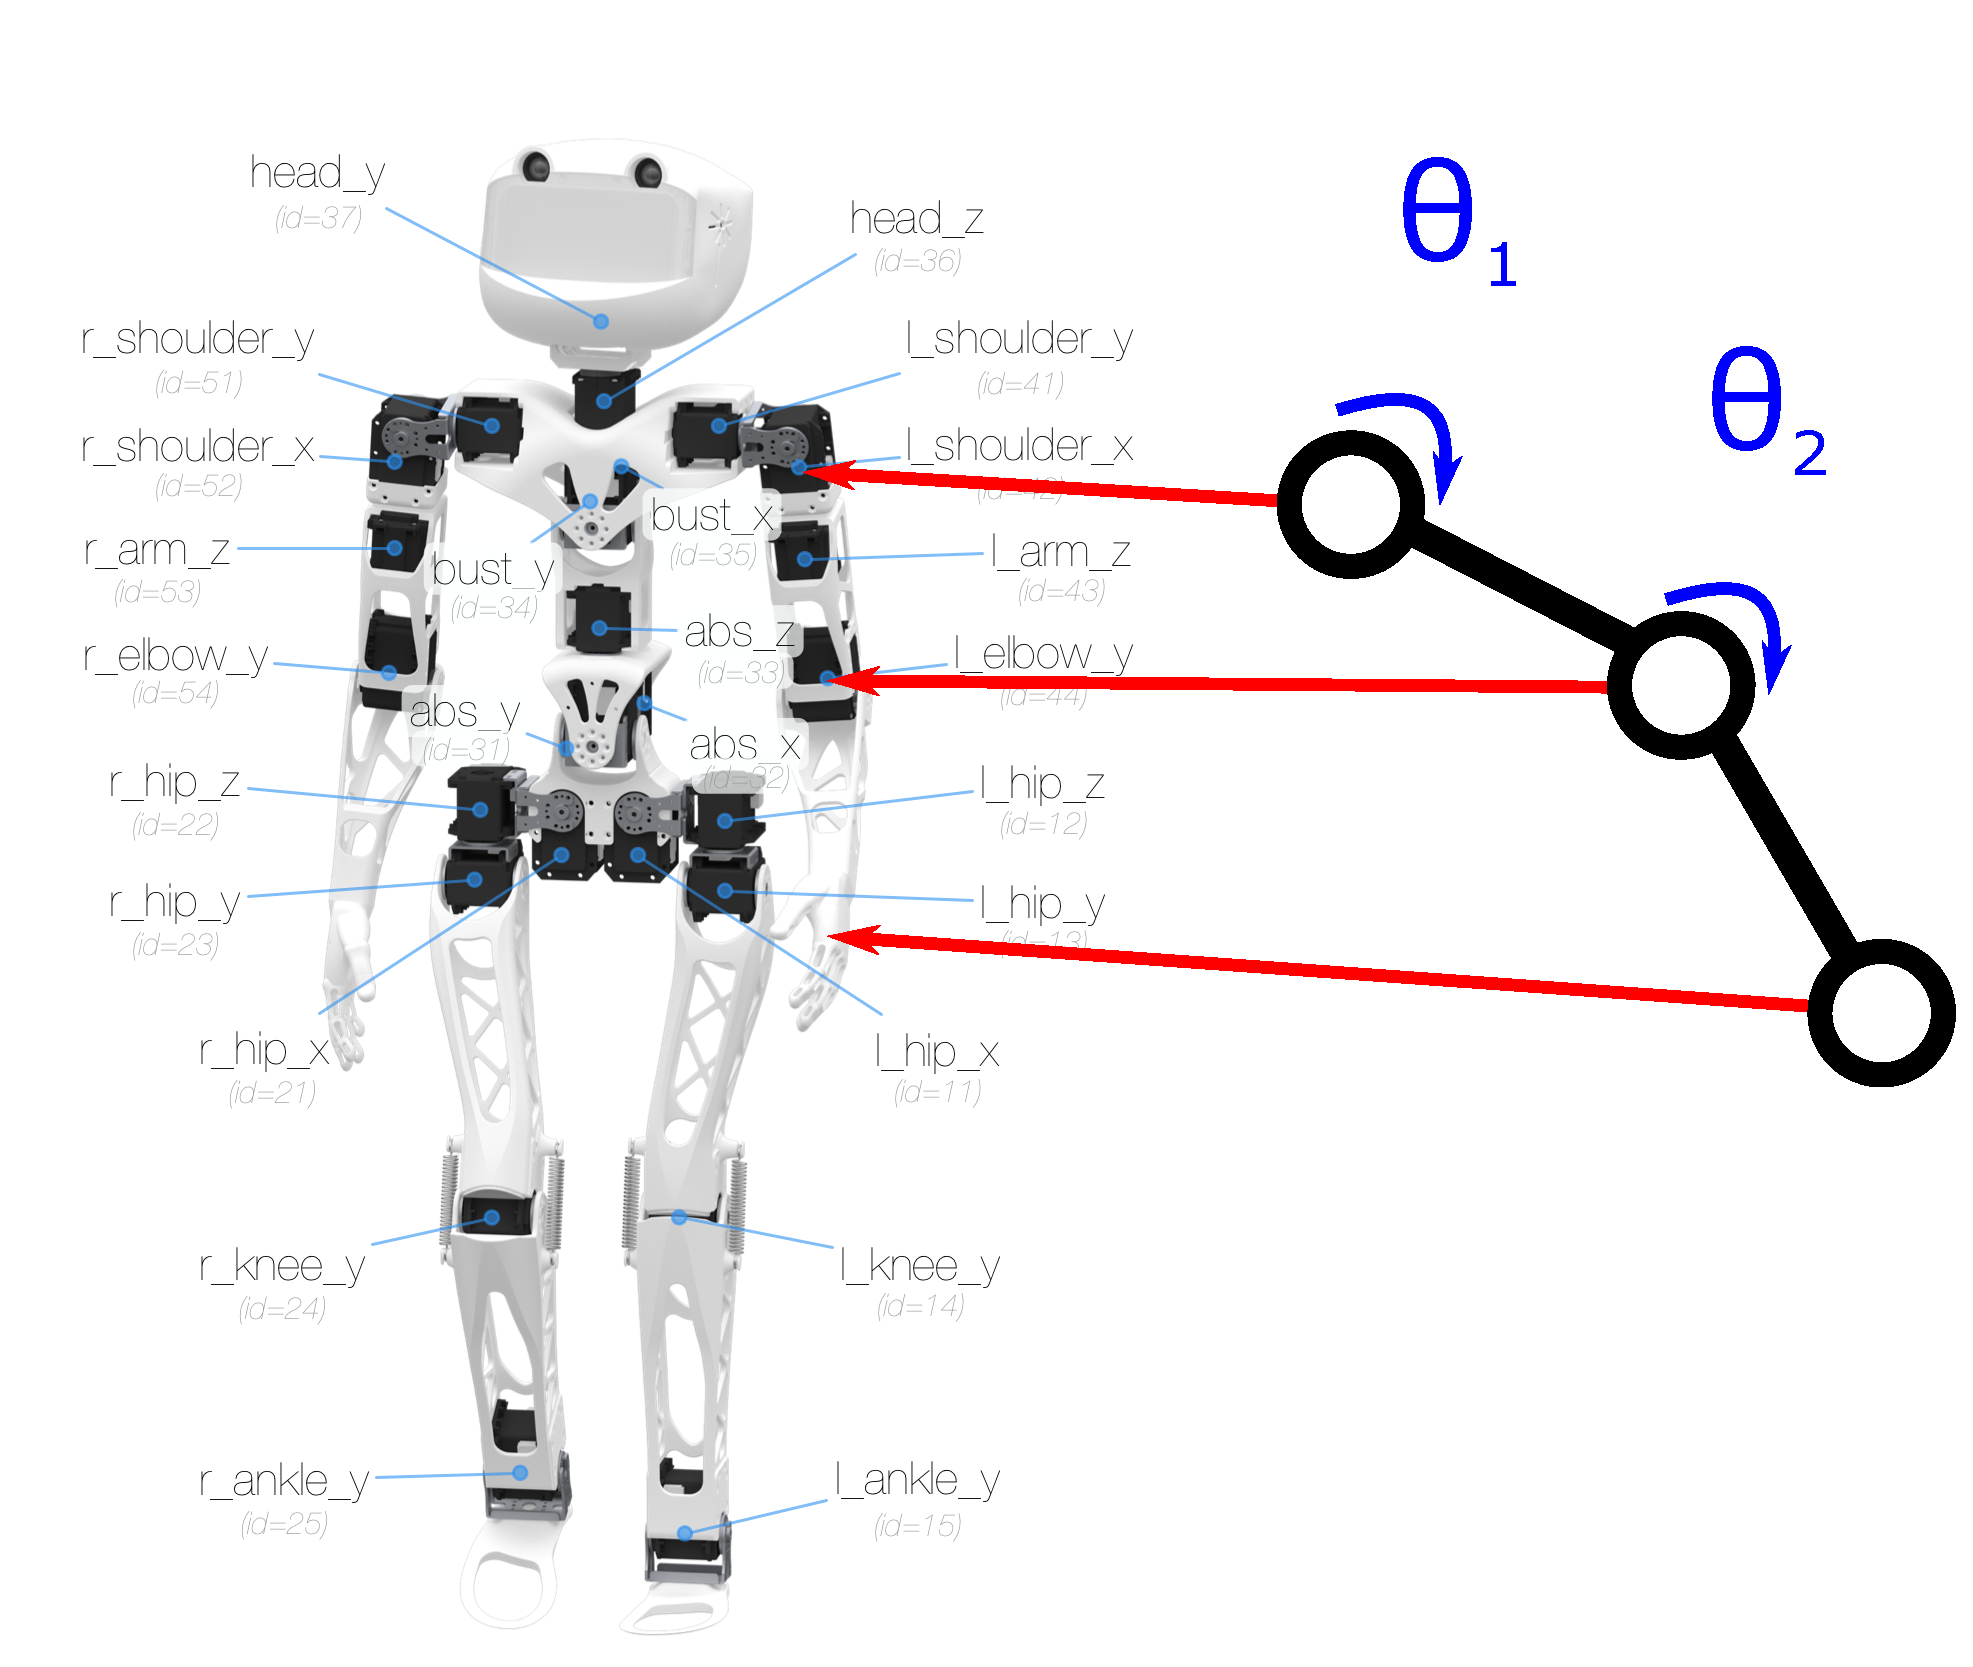
\includegraphics[width=0.7\textwidth]{reportpics/poppy_2dof.eps}
	\caption{Arm Modeling of Poppy}
	\label{fig:poppy_2dof}
\end{figure}

The training follows the learning rules as proposed by Mnih et al. in \cite{mnih2013playing, mnih2015human}, while our Q-Network will not have convolutional layers and is inspired by the works of Lillicrap et al. in \cite{lillicrap2015continuous}. We plan to use an input layer and two hidden layers with each 100 neurons and ReLU activation function. The dimension of the output layer of the Q-Network is 4, i.e. one for each action, and has a linear activation function. In addition, we plan to use the \textit{soft} update rule for the target network as in \cite{lillicrap2015continuous}. Regarding the \ac{DQN} algorithm we aim for a modularized and asynchronous implementation, as visualized in Fig. \ref{fig:async} and inspired by \cite{nair2015massively, mnih2016asynchronous}. In this way, we can interact with different environments in parallel, using seperate threads, and collect more distinct experience samples $e_t$ at timestep $t$ in the form:
\begin{equation}
e_t = [s_t, a_t, r_t, s_{t+1}, terminal]
\end{equation} 
where $s$ is the state of the agent, $a$ the action selected by the agent, $r$ the reward signal according to the distance when arrived at state $s_{t+1}$. The boolean variable $terminal$ denoted if the episode finished after this experience sample and is needed for the Q-learning update rules in the terminal state. \\

\begin{figure}
	\centering
	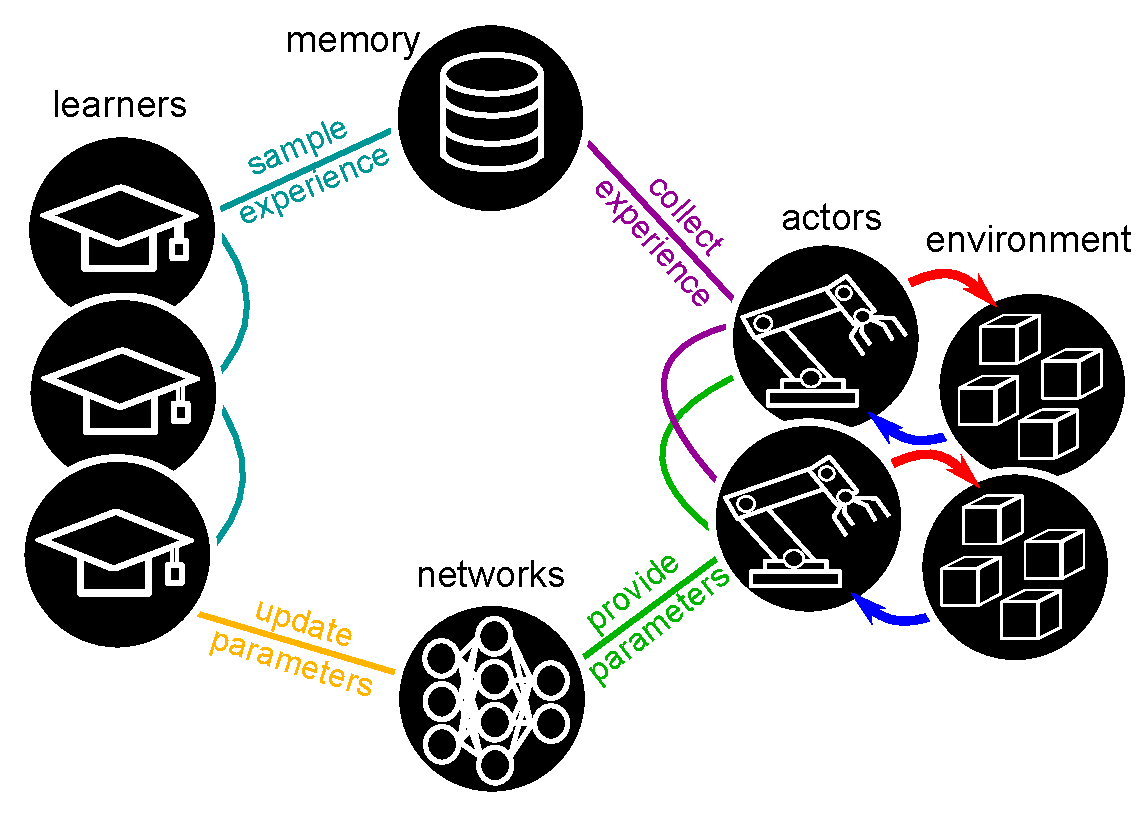
\includegraphics[width=0.6\textwidth]{reportpics/async_e.eps}
	\caption{Asynchronous architecture for Deep Reinforcement Learning}
	\label{fig:async}
\end{figure}

Finally, we noticed that $\epsilon$-greedy is not a good exploration policy in robotics and we will try to guide the robot arm into the goal direction by using \ac{IK}. The main idea of this guidance of the actions is to show the robot almost correct experiences and to let the agent improve itself around this guidance by randomly selecting other actions. These random actions might improve the policy and the agent's behavior could show better performance than the guidance originally taught to the agent. In detail, the exploration will not be fully $\epsilon$-greedy, but $50\%$  $\epsilon$-greedy and $50\%$ \acp{IK} guided. The \acp{IK} guidance is done in the following way. The joint angle velocities $\delta \vec{\theta}$ are computed by:
\begin{equation}
\delta \vec{\theta} = J^{-1} \cdot (\vec{x}_{goal} - \vec{x}_{arm})
\end{equation}
where $J$ is the Jacobian matrix of the robot arm at joint angles $\vec{\theta}$.\\
Then, the motor to control is determined by selecting the motor with the larger joint angle velocity:
\begin{equation}
\argmax_{i \in \{1,2\}}(\delta \theta_1, \delta \theta_2)
\end{equation}
Finally, the action is determined by the motor $i$ to move and the sign of the respective $\delta \theta_i$ in order to decide the direction $\pm1\degree$.

\chapter*{Draft of a Project Plan}

\begin{enumerate}
\item Set up the simulation (done)
\item Use the inverse kinematics as a base controller in simulation (done)
\item Use the inverse kinematics as a base controller on the robot
\item Implement the \ac{DQN} algorithm (done)
\item Include the simulation into \ac{DQN} framework
\item Train the Q-Network and tune hyperparameters
\item Try the Q-Network on the real robot
\item Optional features: vision for goal detection, draw triangle or other shapes, use both arms, etc.
\end{enumerate}


%_______________________________________________________________

%_____Abbildungsverzeichnis_____________________________________
%\cleardoublepage
%\addcontentsline{toc}{chapter}{List of Figures} 
%\listoffigures 	 %Abbildungsverzeichnis
%_______________________________________________________________

%_____Literaturverzeichnis______________________________________
\cleardoublepage
\addcontentsline{toc}{chapter}{Bibliography}
\bibliography{ref}
\bibliographystyle{plain}
%__________________________________________________________

%_____Anhang________________________________________________
%\cleardoublepage
%\appendix
%\appendixpage
%\addappheadtotoc

%Term definitions
\section*{List of Acronyms}
\begin{acronym}[VBLAST]
\acro{DQN}{Deep Q-Network}
\acro{DRL}{Deep Reinforcement Learning}
\acro{IK}{Inverse Kinematic}
\acro{NN}{Neural Network}
\acro{RL}{Reinforcement Learning}  
\acro{TD}{Temporal Difference}
\end{acronym}


\end{document}
